\chapter{Spatial Transformations for the Computations of the Log-composition: SE(2) and SVF}\label{ch:spatial_transformations}


\begin{flushright}
	\emph{Every working mathematician knows that if one does not control oneself (best of all by examples), then after some ten pages half of all the signs in formulae will be wrong and twos will find their way from denominators into numerators. \\ -V.I. Arnold}
\end{flushright}

In the previous chapter we have introduced some essential mathematical tools for the numerical computation of the log-composition. They can be applied for several groups of transformation. In this research we show how they behave on two selected groups:
\begin{enumerate}
	\item[SE(2) -] The group of rigid body transformation of the plane (any combination of bi-dimensional rotations and translations) is the optimal playground to test the numerical methods introduced so far. Here all the closed form can be derived analytically, and therefore a ground truth is always available for comparisons. A representation of this Lie group as a subgroup of the real linear group $GL(2)$, with corresponding Lie algebra will be provided, with all of the closed form of the numerical computations presented in this research.
	\item[SVF -] The subgroup of the set of diffeomorphisms parametrized by SVF, is the second group used to test the numerical methods here presented for the computation of the log-composition. Each one can be applied for the composition of SVF in the diffeomorphic demons and for the log-demons. In this case we do not know any closed form, but if we consider an improper norm in the space of transformation we still have a method to compare SVF and assess the quality of the results.
\end{enumerate}

\noindent
Since each of the theoretical elements at the core of the Lie group theory, depends strongly on the transformations considered, in this chapter we will see how they can be applied for the cases of SE(2) and the Lie group of diffeomorphisms parametrized with stationary velocity fields.

\section{The Lie Group of Rigid Body Transformations}\label{se:rigid_body_transformations}
% group
Each element of the group of rigid body transformation (or euclidean group) $SE(2)$ can be computed as the consecutive application of a rotation and a translation applied to any point $(x,y)^T$ of the plane:
\begin{align*}
\left (  
\begin{array} {c }
X \\
Y
\end{array}
\right )  
= 
R(\theta)
\left (  
\begin{array} {c }
x \\
y
\end{array}
\right ) 
+
t
=
\left (
\begin{array} {c c }
\cos(\theta) & - \sin(\theta) \\
\sin(\theta) & \cos(\theta) 
\end{array}
\right )
\left (  
\begin{array} {c }
x \\
y
\end{array}
\right ) 
+
\left (  
\begin{array} {c }
t_x \\
t_y
\end{array}
\right ) 
\end{align*}
where the rotation matrix defined by $\theta$ belongs to the special orthogonal group $SO(2)$.\\
We can represent the elements of $SE(2)$ in two different form: as ternary vector (restricted form) 
\begin{align*}
SE(2)^{v} 
:=
\{ (\theta, t_x, t_y) \mid \theta \in [0, 2\pi),   t_x, t_y \in\mathbf{R}^2  \}
\end{align*}
or with matrices (matrix form)
\begin{align*}
SE(2) 
:= 
\left \{
\left (
\begin{array} {c c }
R(\theta) & t \\
0 & 1 
\end{array}
\right )
=
\left (
\begin{array} {c c c }
\cos(\theta) & - \sin(\theta)& t_{x} \\
\sin(\theta) & \cos(\theta) & t_{y}\\
0 & 0 &  1
\end{array}
\right )
\mid
\theta \in  [0, 2\pi), (t_x, t_y) \in\mathbf{R}^2
\right \}
\end{align*}
The group $SE(2)$ it is a manifold with a differentiable structure compatible with the operation of composition, whose Lie algebra is given in matrix form by (see \cite{hall2015lie, gallier2011geometric} for an introduction).
\begin{align*}
\mathfrak{se}(2) := 
\left \{
\left (
\begin{array} {c c }
dR(\theta) & dt \\
0 & 0
\end{array}
\right )
=
\left (
\begin{array} {c c c }
0 & -\theta &  dt_{x} \\
\theta & 0 & dt_{y} \\
0& 0 & 0
\end{array}
\right )
\mid
\theta \in  [0, 2\pi), (tx, ty) \in\mathbf{R}^2
\right \}
\end{align*}
and it is indicated with $\mathfrak{se}(2)^{v}$ in its vector form.\\

Given $r$, element of $SE(2)$ with $\theta\neq 0$. Its image with the Lie group logarithm is
\begin{align*}
\log(r)
&=
\sum_{k=1}^{\infty} (-1)^{k+1}~\frac{(r - I)^k}{k}
=
\left (
\begin{array} {c c }
dR(\theta) & L(\theta)t \\
0 & 1 
\end{array}
\right )
\\
&=
\left (
\begin{array} {c c c}
0   & - \theta& \frac{\theta}{2} (\frac{\sin(\theta)}{1-\cos(\theta)} t_x + t_y )\\
\theta & 0     & \frac{\theta}{2} (- t_x + \frac{\sin(\theta)}{1-\cos(\theta)} t_y )\\
0 & 0 &  0
\end{array}
\right )
\end{align*}
where therefore 
\begin{align*}
dR(\theta) = 
\left (
\begin{array} {c c }
0 & -\theta \\
\theta & 0 
\end{array}
\right )
\qquad \qquad 
L(\theta) = 
\frac{\theta}{2}
\left (
\begin{array} {c c }
\frac{\sin(\theta)}{1-\cos(\theta)} & 1 \\
-1 & \frac{\sin(\theta)}{1-\cos(\theta)}
\end{array}
\right )
\end{align*}
On the way back, the exponential of $dr \in \mathfrak{se}(2)$ is given by:
\begin{align*}
\exp(dr)
&=
\sum_{k=1}^{\infty} \frac{dr^{k}}{k!}
=
\left (
\begin{array} {c c }
R(\theta) & L(\theta)^{-1}t \\
0 & 1 
\end{array}
\right )
\\
&=
\left (
\begin{array} {c c c}
\cos(\theta)   & - \sin(\theta)& \frac{1}{\theta} (\sin(\theta)dt_x - (1-\cos(\theta)) dt_y )\\
\sin(\theta) & \cos(\theta)     & \frac{1}{\theta} (- (1-\cos(\theta))dt_x + \sin(\theta) dt_y )\\
0 & 0 &  1
\end{array}
\right )
\end{align*}
where
\begin{align*}
L(\theta)^{-1} = 
\frac{1}{\theta}
\left (
\begin{array} {c c }
\sin(\theta) & -(1-\cos(\theta)) \\
(1-\cos(\theta)) & \sin(\theta)
\end{array}
\right )
\end{align*}
When $\theta$ is zero, $R(\theta)$ and $dR(\theta)$ coincide with the identity, and the transformation results in a translation. For proof and further details see for example \cite{gallier2011geometric} \cite{hall2015lie}.\\

At this point it is important to notice that: 
\begin{enumerate}
	%infinite series 
	\item The infinite series of matrices  do not raises any theoretical issues, since the sum is defined in the group as subset of a bigger algebra that contains both the Lie group and the Lie algebra. The infinite series of matrices appears to be the natural way to back and forth from the group to the algebra. A second door to passing from one structure to the other, when $\mathbf{r}$ has a little rotation element appears to be provided by the following approximations:
	\begin{align*}
	\exp(r) \simeq I + r
	\qquad 
	\log(dr) \simeq dr - I
	\end{align*}
	In fact for little $\theta$, $\sin(\theta) \simeq \theta$, $\cos(\theta) \simeq 0 $ and $ L(\theta)^{-1} \simeq I$.
	% restriction of the domain.
	\item The map $\exp$ is not well defined over its whole domain $\mathfrak{se}(2)$. Given two elements $(\theta_0, dt_0x, dt_0y)$ and $(\theta_1, dt_1x, dt_1y)$, they have the same image with $\exp$ function if the two following conditions are both satisfied:
	\begin{enumerate}
		\item[i)] Exists an integer $k$ such that $\theta_0 = \theta_1 + 2k\pi$.
		\item[ii)] the translation $(dt_0x, dt_0y)$ coincides with $(dt_1x, dt_1y)$ up to a factor $\frac{\theta_0 \mod 2\pi}{\theta_1}$.
	\end{enumerate}
	To have a bijective correspondence we have to restrict the domain of $\exp$ to a space where if $\exp(\theta_0, dt_0x,d t_0y) = \exp(\theta_1, dt_1x, dt_1y)$ it implies  $(\theta_0, dt_0x, dt_0y) = (\theta_1, dt_1x, dt_1y)$.
	It can be easy to prove that the sought space is the quotient of $\mathfrak{se}(2)$ over the equivalence relation $\sim$, defined as 
	\begin{align*}
		(\theta_0, dt_0x, dt_0y & ) \sim (\theta_1, dt_1x, dt_1y)
		\\
		~^{\text{def}}&\iff
		\\
		\exists k\in\mathbb{Z} \mid \theta_0 = \theta_1 + 2k\pi 
		&~\text{ and }~
		(dt_0x, dt_0y) = \frac{\theta_0 \mod 2\pi}{\theta_1}(dt_1x, dt_1y)
	\end{align*}
	The new algebra defined by the set of equivalence classes of this relation is indicated - with the standard convention, see \cite{artin2011algebra} - with $\mathfrak{se}(2)/\sim$. With this restriction of the domain$\exp$ is a bijection having $\log$ as its inverse.
	What said so far can be summarize in the following commutative diagram:
	
	\[
	\begindc{\commdiag}[40]
	\obj(55,15)[u]{$\mathfrak{se}(2)/\sim $}
	
	%rightside
	\obj(35,30)[se]{$\mathfrak{se}(2)$}
	\obj(35,0)[SE]{$SE(2)$}
	
	% oblique right
	\mor{se}{u}{$\pi$} [\atright,\surjectivearrow]
	\mor{u}{SE}{$\exp$}
	% vertical
	\mor{SE}{se}{$\log$} 
	
	
	\enddc
	\]
	
	and with the schematic figure \ref{fig:restriction_exp_se2}.
	
	\begin{figure}[!ht]
		\centering
		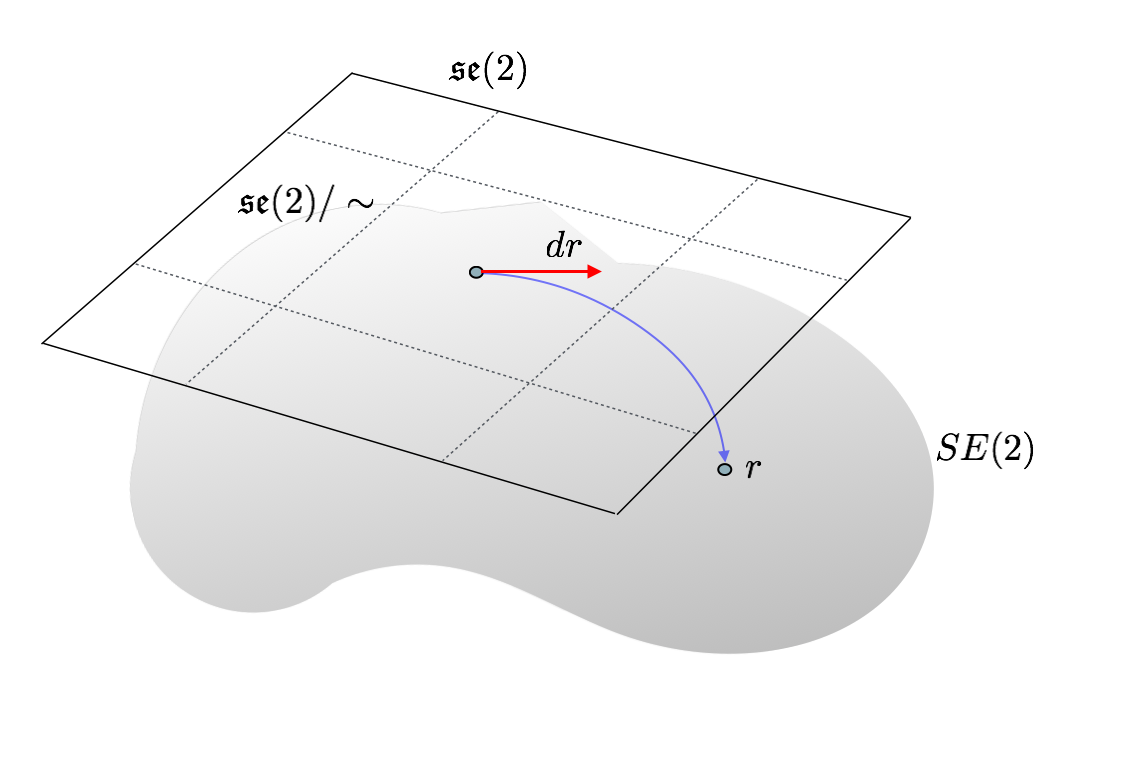
\includegraphics[scale=0.35]{figures/exp_se2.png}
		\caption{The Lie algebra $\mathfrak{se}(2)/\sim$ defined as the quotient of the Lie algebra $\mathfrak{se}(2)$ over the equivalence relation $\sim$ is in bijective correspondence with $SE(2)$.}
		\label{fig:restriction_exp_se2}
	\end{figure}
	
\end{enumerate}

\noindent
The log composition of two elements in $dr_0 = (\theta_0, dt_0x, dt_0y), dr_1 = (\theta_1, dt_1x, dt_1y) \in \mathfrak{se}(2)/\sim$ is provided as a direct applications of the definitions provided for this case. It results
\begin{align*}
dr_0 \oplus dr_1 =  \log(\exp(dr_0)\circ \exp(dr_1))
\end{align*}













% % % % % % % % % % % % % % % % % % % % % % % % % % % % % % % % % % % %
% % % % % % % % % % % % % % % % % % % % % % % % % % % % % % % % % % % %
% % % % % % % % % % % % % % % % % % % % % % % % % % % % % % % % % % % %
% % % % % % % % % % % % % % % % % % % % % % % % % % % % % % % % % % % %
% % % % % % % % % % % % % % % % % % % % % % % % % % % % % % % % % % % %
% % % % % % % % % % % % % % % % % % % % % % % % % % % % % % % % % % % %
\section{The Set of Stationary Velocity Fields}





%% vect function for Lie algebra: vectorization
%The vectorization map transform each matrix $A = \{a_{i,j}\}$ of $M_{3}(\mathbb{R})$ in a $n\times n$ dimensional vector:
%\begin{align*}
%\text{vect} : M_{3}(\mathbb{R}) & \longrightarrow  \text{rbt} 
%\end{align*}
%%
%%Its restriction is an isomorphism between $\text{rbt} $ and $SE(2) $ are isomorphic through the restriction of the vectorization map
%%\begin{align*}
%%\text{vect}_{r} : \mathfrak{se}(2) & \longrightarrow  \text{rbt} 
%%\\
%%\left (
%%\begin{array} {c c c }
%%0 & 0 &  1\\
%%\cos(\theta) & - \sin(\theta)& t_{x} \\
%%\sin(\theta) & \cos(\theta) & t_{y}
%%\end{array}
%%\right )
%%&\longmapsto  (\theta, t_{x}, t_{y}) 
%%\end{align*}
% two doors to going from the lie group to the lie algebra
% passage from restricted to matrix form
%Aimed to restrict the domain... we provide explicitly the bijections to pass in both structure from the vector to the matrix form and vice versa:
%\begin{align*}
%\rho_{SE(2)}: SE(2)^{v} &\longrightarrow SE(2)\\
%(\theta, tx, ty) 
%& \longmapsto
%\left (
%\begin{array} {c c c }
%\cos(\theta) & - \sin(\theta)& tx \\
%\sin(\theta) & \cos(\theta) & ty\\
%0 & 0 &  1
%\end{array}
%\right )
%\end{align*}
%
%\begin{align*}
%\rho_{\mathfrak{se}(2)} : \mathfrak{se}(2)^{v}&\longrightarrow  \mathfrak{se}(2)\\
%(\theta, dtx, dty) 
%& \longmapsto
%\left (
%\begin{array} {c c c }
%0 & -\theta & dtx \\
%\theta & 0 & dty\\
%0 & 0 &  1
%\end{array}
%\right )
%\end{align*}



%
%
%
%A rigid body transformation in a normed vector space is a transformation that preserves distances. The set of rigid body transformations is constructed as any combination of rotations, translations and reflection, and forms the euclidean group $E(2)$. For 2d rigid registration usually reflections are not required and so we restrict our attention to the special euclidean group $SE(2)$.  We are interested in two things about them: their expression in matrix form, and the Lie group and the Lie algebra structures involved. \\
%We denote denoted with $M_{3}(\mathbb{R})$ the set of all of the $3\times 3$ matrices with real entries . 
%Its subset, defined by all the matrices with non-zero determinant, and thus by all the invertible matrices, is denoted with $GL_3 (\mathbb{R})$. A \emph{matrix group} is any proper or improper subgroup of  $GL_3 (\mathbb{R})$.
%The group of 2d rigid body transformation 
%\begin{align*}
%\mathbb{G} =
%\{ (\theta, tx, ty) \mid \theta \in [0, 2\pi),   tx, ty \in\mathbf{R}^2  \}
%\end{align*}
%using matrices, so as a subgroup of $GL_3 (\mathbb{R})$.
%Rotation in the plane can be expressed using matrix of the orthogonal group $SO(2)$, linear subgroup of $GL_2 (\mathbb{R})$, so that rotations' actions on planes' points are simply defined as a product: 
%\begin{align*}
%SO(2) = 
%\left \{
%\left (
%\begin{array} {c c }
%\cos(\theta) & - \sin(\theta) \\
%\sin(\theta) & \cos(\theta) 
%\end{array}
%\right )
%\mid
%\theta \in  [0, 2\pi)
%\right \}
%\end{align*}
%To include the translation we can add its $(tx, ty)^{T}$ parameter to the action of the rotation over the initial point $(x_{i}, y_{i})^{T}$ to obtain the transformed $(x_{t}, y_{t})^{T}$. So each element of the group $\mathbb{G}$ act over $\mathbf{R}^2$ as
%\begin{align*}
%\left (  
%\begin{array} {c }
%x_{t} \\
%y_{t}
%\end{array}
%\right ) 
%= 
%\left (
%\begin{array} {c c }
%\cos(\theta) & - \sin(\theta) \\
%\sin(\theta) & \cos(\theta) 
%\end{array}
%\right )
%\left (  
%\begin{array} {c }
%x_{i} \\
%y_{i}
%\end{array}
%\right ) 
%+
%\left (  
%\begin{array} {c }
%tx \\
%ty
%\end{array}
%\right ) 
%\end{align*}
%Another way to express rigid body transformation group's elements is to include the translation in a bigger matrix, subgroup (not linear, since the translation is not linear) of $GL_3 (\mathbb{R})$. This is defined as the group $SE(2)$:
%\begin{align*}
%SE(2) = 
%\left \{
%\left (
%\begin{array} {c c c }
%\cos(\theta) & - \sin(\theta)& t_{x} \\
%\sin(\theta) & \cos(\theta) & t_{y}\\
%0 & 0 &  1
%\end{array}
%\right )
%\mid
%\theta \in  [0, 2\pi), (tx, ty) \in\mathbf{R}^2
%\right \}
%\end{align*}
%Expressed in this way the matrices act on the point of the plane represented as the elements of the vector space $\{1 \} \times \mathbf{R}^2$.\\ 
%The passage between the restricted form $\mathbb{G} $ and $SE(2)$ is defined by the injection:
%\begin{align*}
%\rho^{v} : \mathbb{G} &\longrightarrow   SE(2)\\
%(\theta, tx, ty) 
%& \longmapsto
%\left (
%\begin{array} {c c c }
%\cos(\theta) & - \sin(\theta)& tx \\
%\sin(\theta) & \cos(\theta) & ty\\
%0 & 0 &  1
%\end{array}
%\right )
%\end{align*}
%We are now interested the Lie algebra of the Lie group $SE(2)$. 
%%In general a matrix Lie group is any complete subgroup of $GL(n,\mathbb{R})$ while its Lie algebra is a particular subset (not necessarily a group) of $GL(n,\mathbb{R})$. 
%%\begin{prop}\label{pr:matrixLiealgebra}
%%	Be $\mathbb{G}$ a matrix Lie group.
%%	\begin{itemize}
%%		\item[a)] If $\mathbb{G} = GL(n,\mathbb{R})$ then $T_{e}\mathbb{G} = M(n,\mathbb{R})$.  
%%		\item[b)] If $\mathbb{G} \subseteq GL(n,\mathbb{R})$ then $T_{e}\mathbb{G} \subseteq M(n,\mathbb{R})$.
%%	\end{itemize}
%%\end{prop}
%%\begin{proof}
%%	since $det$ is a continuous function we have that 
%%	\begin{align*}
%%	\forall X \in M(n,\mathbb{R})~~ \exists &\eta > 0 \text{ such that } \forall t \in(-\eta , \eta) \\
%%	&det(I+tX) \neq 0
%%	\end{align*}
%%	where $I$ is the identity matrix. If we consider the path
%%	\begin{align*}
%%	\gamma : [0,1] & \longrightarrow  GL(n,\mathbb{R}) \\
%%	t &\longmapsto I+tX
%%	\end{align*}
%%	as the path joining $I$ and $X$, it follows
%%	\begin{align*}
%%	\frac{d }{dt}(I+tX)~\Bigr|_{t = 0}  = X \in M(n,\mathbb{R})
%%	\end{align*}
%%\end{proof}
%It is defined as:
%\begin{align*}
%\mathfrak{se}(2) = 
%\left \{
%\left (
%\begin{array} {c c c }
%0 & -\theta &  dt_{x} \\
%\theta & 0 & dt_{y} \\
%0& 0 & 1
%\end{array}
%\right )
%\mid
%\theta \in  [0, 2\pi), (tx, ty) \in\mathbf{R}^2
%\right \}
%\end{align*}
%Expressing $r\in SE(2)$ as:
%\begin{align*}
%\mathbf{r} = 
%\left (
%\begin{array} {c c }
%R(\theta) & t \\
%0 & 1 
%\end{array}
%\right )
%\qquad
%R(\theta) \in SO(2) 
%\quad
%t \in \mathbb{R}^{2}
%\end{align*}
%for $t$ plane translation and $R(\theta)$ in $SO(2)$, then the element of the Lie algebra can be expressed as:
%\begin{align*}
%d\mathbf{r} 
%= 
%\left (
%\begin{array} {c c }
%dR(\theta) & dt \\
%0 & 1 
%\end{array}
%\right )
%\qquad
%R(\theta) \in SO(2) 
%\quad
%t \in \mathbb{R}^{2}
%\end{align*}
%Both $SE(2)$ and $\mathfrak{se}(2)$ are in bijective correspondence with $\mathbb{G}$, and both are subset of the bigger algebra of, The algebra $\mathfrak{se}(2)$ do not form a group with the operation of composition, but it is provided with the lie bracket defined by the commutator:
%\begin{align*}
%[d\mathbf{r}, d\mathbf{s}] = d\mathbf{r} d\mathbf{s} - d\mathbf{s} d\mathbf{r}
%\end{align*}
%The Lie logarithm between Lie group and Lie algebra is given by:
%\begin{align*}
%\log : \mathfrak{se}(2) & \longrightarrow SE(2)
%\\
%\left (
%\begin{array} {c c }
%R(\theta) & t \\
%0 & 1 
%\end{array}
%\right )
%&\longmapsto  
%\left (
%\begin{array} {c c }
%dR(\theta) & dt \\
%0 & 1 
%\end{array}
%\right )
%\end{align*}
%Where 
%\begin{align*}
%dR(\theta) = 
%\left (
%\begin{array} {c c }
%0 & -\theta \\
%\theta & 0 
%\end{array}
%\right )
%\end{align*}
%and $dt = L(\theta)t$ for 
%\begin{align*}
%L(\theta) = 
%\frac{\theta}{2}
%\left (
%\begin{array} {c c }
%\frac{\sin(\theta)}{1-\cos(\theta)} & 1 \\
%-1 & \frac{\sin(\theta)}{1-\cos(\theta)}
%\end{array}
%\right )
%\end{align*}
%The inverse function, Lie exponential is given by:
%\begin{align*}
%\exp : SE(2) & \longrightarrow \mathfrak{se}(2) 
%\\
%\left (
%\begin{array} {c c }
%dR(\theta) & dt \\
%0 & 1 
%\end{array}
%\right )
%&\longmapsto  
%\left (
%\begin{array} {c c }
%R(\theta) & t \\
%0 & 1 
%\end{array}
%\right )
%\end{align*}
%where $t = L(\theta)^{-1}dt$ for 
%\begin{align*}
%L(\theta)^{-1} = 
%\frac{1}{\theta}
%\left (
%\begin{array} {c c }
%\sin(\theta) & -(1-\cos(\theta)) \\
%(1-\cos(\theta)) & \sin(\theta)
%\end{array}
%\right )
%\end{align*}





%
%If the tangent space to the group of diffeomorphisms is defined in analogy with the finite dimensional case, it turns out that the exponential map is not a bijection in a local neighborhood of the identity. That means that there are non-trivial elements in the group that are not the image of any tangent vector in the Lie algebra. Taking into account exponential and logarithm implies a restriction in the diffeomorphisms to the image of exp.
%For this reason it is improper to talk about Diffeomorphisms if the Log and exponential maps are taken into account in the framework: in image registration literature it is used instead time varying velocity fields (TVVF), or stationary velocity field (SVF), according to the nature of the differential equation that governs the correspondence between Lie algebra and Lie group. In the case of 
%Therefore considering only a subset of diffeomorphisms that are lost in considering the Log-euclidean framework
%
%... la struttura di gruppo e' comunque recuperata, in modo banale nel caso dei SVF e in modo un po' meno banale nel caso dei TVVF, se si considera il sottogruppo ad un parametro, rispetto al quale l'operazione di composizione e' chiusa e ben definita.
%
%with the exponential map. that Instead of considering all of the diffeomorphisms in the infinite dimensional group on the compact subset $\Omega$ of $\mathbb{R}^d$d, we consider only the diffeomorphisms that are in the image one parameter subgroup. This restriction appears to not have any negative consequences for practical applications, but enable to treat diffeomorphisms, why only subset, the strategy to compute the ground truth.







% %
% \begin{lemma}\label{le:D1equalsD}
%  Given $\varphi_{t}^{\alpha}(e)$, for each $t \in \mathbb{R}$ exists $V^{\beta} \in left\mathfrak{X}(\mathbb{G})$ such that 
%  \begin{align*}
%    \varphi_{t}^{\alpha}(e) = \varphi_{1}^{\beta}(e) 
%  \end{align*}
% \end{lemma}
% %
% Immediate consequence of the previous lemma is:
% \begin{prop}
% Using the above definitions, it follows that
%  \begin{align*}
%   Diff_{1} = \mathbb{G}
%  \end{align*}
% \end{prop} 
% We defined $Diff_{1}$ in order to reflect the lenght of the vectors in $\mathfrak{g}$ immediately over $\mathbb{G}$. This lead to have a sraight correspondence between vectors in the Lie algebra and elements in the Lie group, that we will investigate in the next subsection.



% % % % % % % % % % % % % % % % % % % % % % % % % % % % % % % % % % % % % %
% % SUBSECTION
% % % % % % % % % % % % % % % % % % % % % % % % % % % % % % % % % % % % % % 
%\subsubsection{Metrics in $\text{Diff}(\Omega)$}
%Relying on the Lie algebra tangent structure it is possible to define a family of metrics in the Lie group as follows:
%\begin{align*}
%\text{dist}(p,q) := \euclideanMetric{\mathbf{u}  - \mathbf{v} }_{\mathfrak{g}}
%\end{align*}
%$(\text{Diff}(\Omega), \text{dist})$ is a metric space. For the finite dimensional case if $\mathfrak{g}$ is complete then $(Diff, dist)$ is complete (.... investigate the if it is complete even in the infinite dimensional case!).\\
%It is possible to define sum in the Lie group, compatible with the metric using the sum in the Lie algebra and the function exp and log.
%	\begin{align*}
%	\odot : \text{Diff}(\Omega) \times \text{Diff}(\Omega) & \longrightarrow  \text{Diff}(\Omega)    \\
%	(p, q) &\longmapsto \exp(log(p) + log(q))
%	\end{align*}
%	Note that $log(p) + log(q)$ is an element of the Lie algebra$\mathfrak{g}$ while  $\exp(log(p) + log(q))$ is in $\mathbb{G}$. Following properties hold
%
%	\begin{enumerate}
%		%
%		\item $\odot$ is well defined.
%		%
%		\item Closure of $\odot$ under inverse element: if $p \in \mathbb{G}$ then $p^{-1} \in \mathbb{G}$.
%		%
%		\item Distance is inversion invariant:
%		\begin{align*}
%		\text{dist}(p,q) = dist(p^{-1},q^{-1})
%		\end{align*}
%		%
%		\item Distance is invariant under $\odot$:
%		\begin{align*}
%		\text{dist}(p,q) = dist(p \odot r,q \odot r)
%		\end{align*}
%		%
%		\item The distance is not invariant under the composition of group structure of $\mathbb{G}$:
%		\begin{align*}
%		\text{dist}(p,q) \neq dist(p\circ r,q \circ r)
%		\end{align*}
%		%
%	\end{enumerate}
%	%

%\begin{corollary}
%	Using the 
%	If, with previous notations, the condition (1) is an approximation
%	\begin{align*}
%	\exp_{C}(\frac{\mathbf{k}}{2}) = \exp(\mathbf{\xi})\circ \exp_{M}(\frac{\mathbf{k}}{2}) 
%	\end{align*}
%	for some $ \mathbf{\xi}$ in  $\mathfrak{g}$ such that $\parallel\mathbf{\xi} \parallel < \delta$
%	then the approximation has error
%	\begin{align*}
%	O(\parallel \delta\mathbf{u}^{\parallel} \parallel^{2} )  
%	+ O(\parallel \mathbf{u} + \delta\mathbf{u}\parallel^{3})
%	+ \text{xxx something that must be investigated depending on } \delta
%	\end{align*}
%\end{corollary}
